\begin{mdframed}
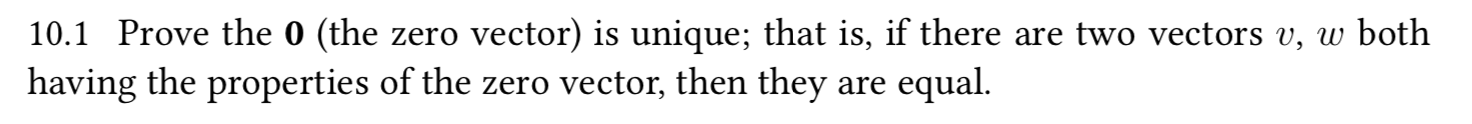
\includegraphics[width=400pt]{img/linear-algebra-kun-pimbook-exercises--6242.png}
\end{mdframed}

The properties of the zero vector are
\begin{enumerate}
\item $\0 + u = u$ for every vector $u$ (additive identity)
\item $a\0 = \0$ for every scalar $a$
\end{enumerate}

\begin{proof}
  Let $a \neq 1$ be a scalar from the field.

  We have $av - v = aw - w$, since both are equal to $\0$. Therefore $v(a - 1) = w(a - 1)$, therefore $v = w$.
\end{proof}

\begin{proof}
  Let $u \neq \0$ be a vector. We have $u + v = u + w = 0$, therefore $v = w$.
\end{proof}

\begin{mdframed}
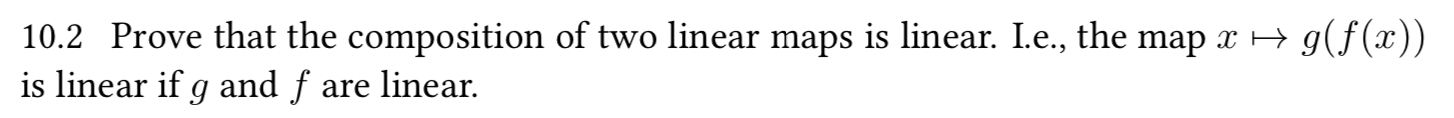
\includegraphics[width=400pt]{img/linear-algebra-kun-pimbook-exercises--f0b5.png}
\end{mdframed}

\begin{proof}
\begin{align*}
  (g \circ f)(ax + by)
  &= g(f(ax + by)) \\
  &= g(af(x) + bf(y)) \\
  &= ag(f(x)) + bg(f(y)) \\
  &= a(g \circ f)(x) + b(g \circ f)(y)
\end{align*}
\end{proof}

